\documentclass[english, aspectratio=169]{beamer}

%style
\mode<presentation>{
	%\usetheme{frankfurt}
	\usetheme{default}
}

%packages
\usepackage[utf8]{inputenc}
\usepackage[english]{babel}
\usepackage{graphicx}
\usepackage{mathtools}
\usepackage{amsmath}
\usepackage{epstopdf}

%
% packages.tex -- packages required by the paper in this directory
%
% (c) 2019 Prof Dr Andreas Müller, Hochschule Rapperswil
%

\usepackage{pgf}
\DeclareUnicodeCharacter{2212}{--}


%Einstellungen Präsentation
\title{VHDL Implementation of Wavelets}
\author{Jonas Gründler \& Nicolas Tobler }
\institute{Mathematisches Seminar 2019}
\date{28.05.2019}

%Bilder
\graphicspath{{images/}}

%Beginn der Präsentation
\begin{document}

%Titelseite
\begin{frame}
\titlepage
\end{frame}

%Inhaltsverzeichnis
\begin{frame}
\frametitle{Contents}
\tableofcontents
\end{frame}

\section{Introduction}

\begin{frame}
	\frametitle{Theory 1}
	"Factoring Wavelet Transforms Into Lifting Steps"\\
	 (by Ingrid Daubechies and Wim Sweldens)\\
	1. Polyphase components
	\begin{equation}
	\begin{aligned}
		x = (x_k)_{k \in Z} \Rightarrow x_e &= (x_{2k})_{k \in Z} \\
		x_o &= (x_{2k+1})_{k \in Z}
		\end{aligned}
	\end{equation}
	where $x_e$ and $x_o$ are closely correlated
\end{frame}

\begin{frame}
\frametitle{Theory 2}
2. Predictor $P$ and difference $d$
\begin{equation}
d = x_e - P(x_o)
\end{equation}
it follows 
\begin{equation}
	x_e = P(x_o) + d
\end{equation}
and
\begin{equation}
	d_k = x_{2k+1} - (x_{2k} + x_{2k+2})/2
\end{equation}\\
Computing a prediction and recording is called a lifting step.
\end{frame}
\begin{frame}
\frametitle{Theory 3}
3. Update $U$ 
\begin{equation}
	s = x_e + U(d)
\end{equation}
in reverse
\begin{equation}
x_e = s -U(d)
\end{equation}

This way $x_o$ can be recovered from $x_e$.
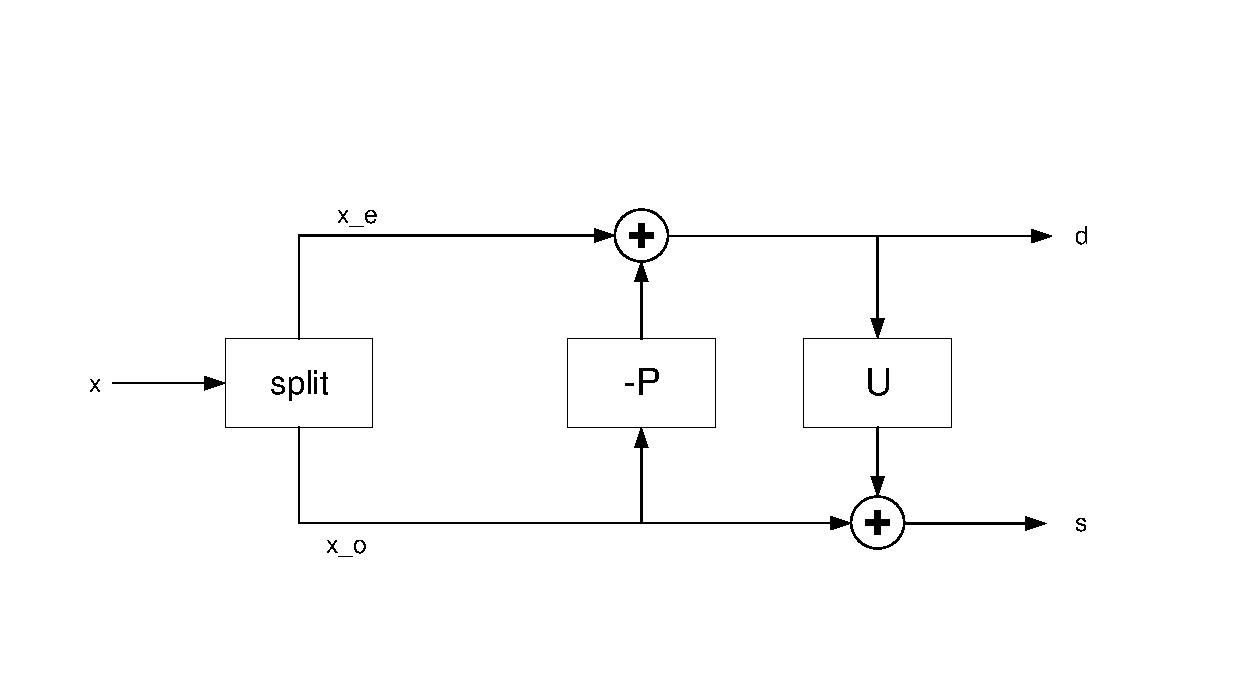
\includegraphics[scale=0.5]{lifting_step.pdf}
\end{frame}
\begin{frame}
\frametitle{Theory 4}
	This technique is then adapted for the Wavelet Transform: 
	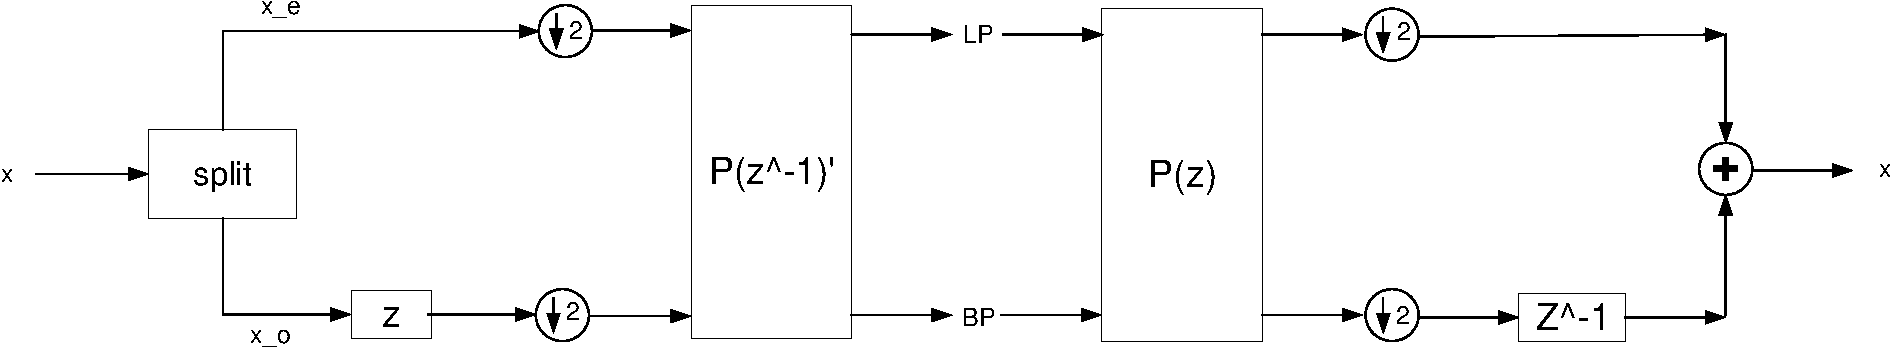
\includegraphics[scale=0.3]{lifting_step_wavelet.pdf}\\
	where $P(z^{-1})^t$ and $P(z)$ depend on the Wavelet.
	
\end{frame}



\begin{frame}
\frametitle{Idea}

\begin{figure}
	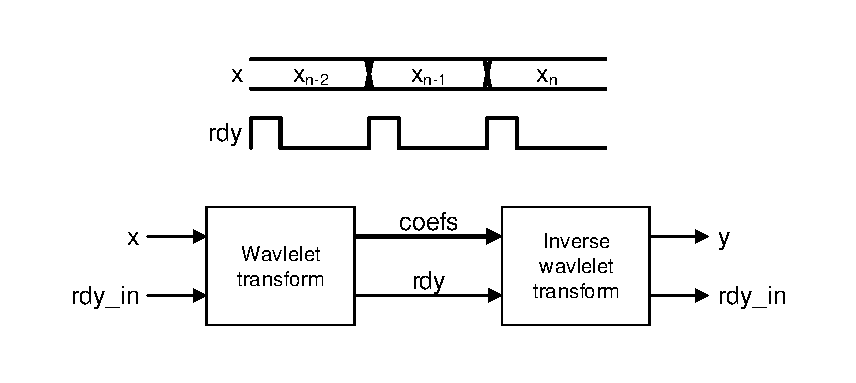
\includegraphics[scale=0.7]{idea.pdf}
\end{figure}
\end{frame}


\section{Architecture}
\begin{frame}
\frametitle{Design considerations}

\begin{figure}
	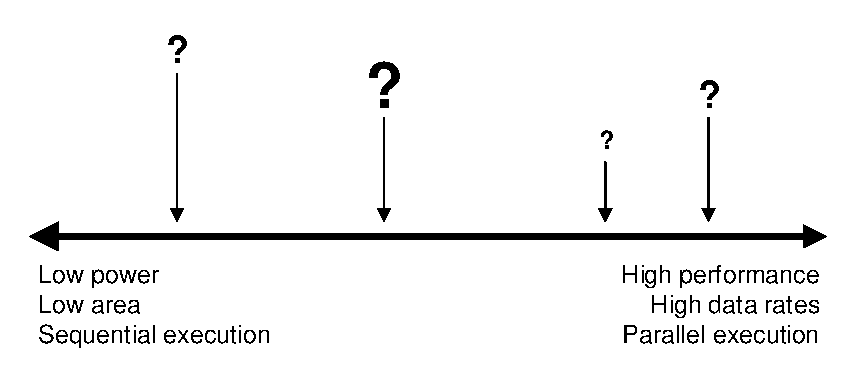
\includegraphics[scale=0.7]{design_considerations.pdf}
\end{figure}

\begin{itemize}
	
	\item[$\bullet$] Application

	\item[$\bullet$] Expensive components
	\begin{itemize}
		\item[-] Multipliers
		\item[-] Memory cells
	\end{itemize}
	
\end{itemize}
\end{frame}


\begin{frame}
\frametitle{Haar}

	\begin{figure}
		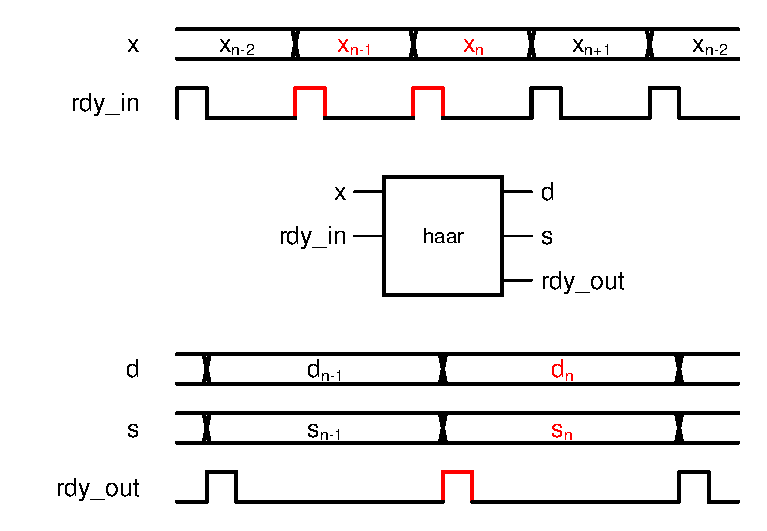
\includegraphics[scale=0.7]{haar.pdf}
	\end{figure}

\end{frame}

\begin{frame}
\frametitle{Inverse haar}

	\begin{figure}
		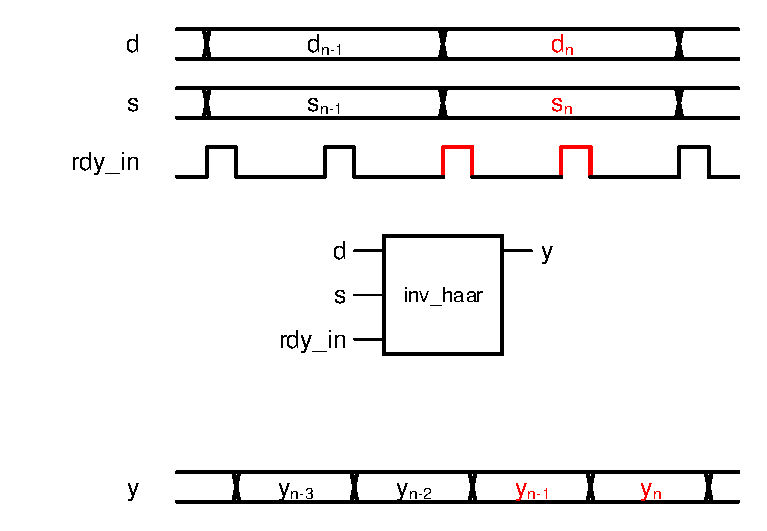
\includegraphics[scale=0.7]{inv_haar.pdf}
	\end{figure}

\end{frame}




\begin{frame}
\frametitle{Branching}

\begin{figure}
	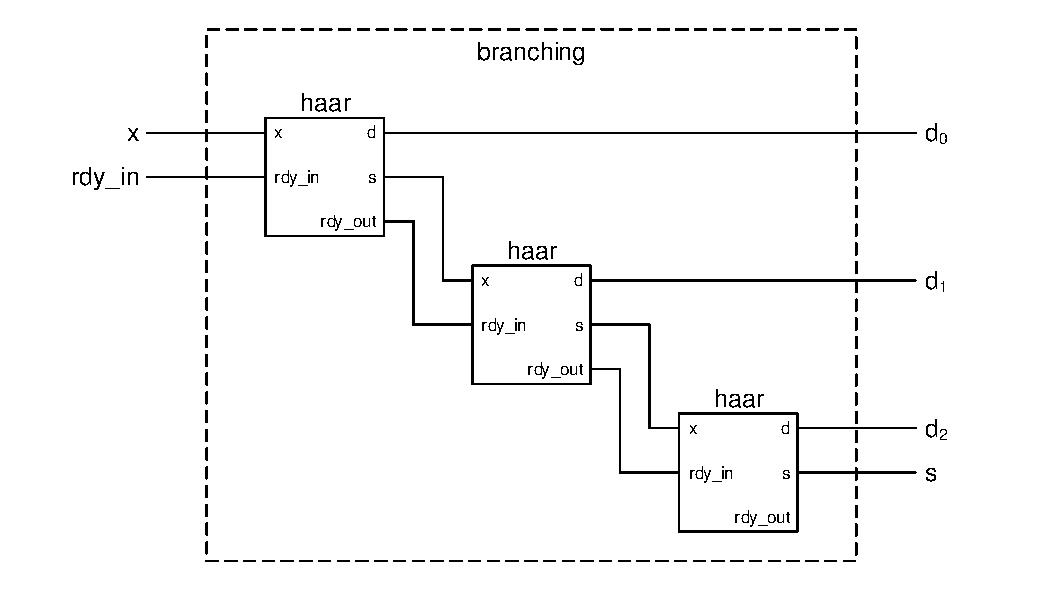
\includegraphics[scale=0.7]{branching.pdf}
\end{figure}

\end{frame}


\begin{frame}
\frametitle{Inverse branching}

\begin{figure}
	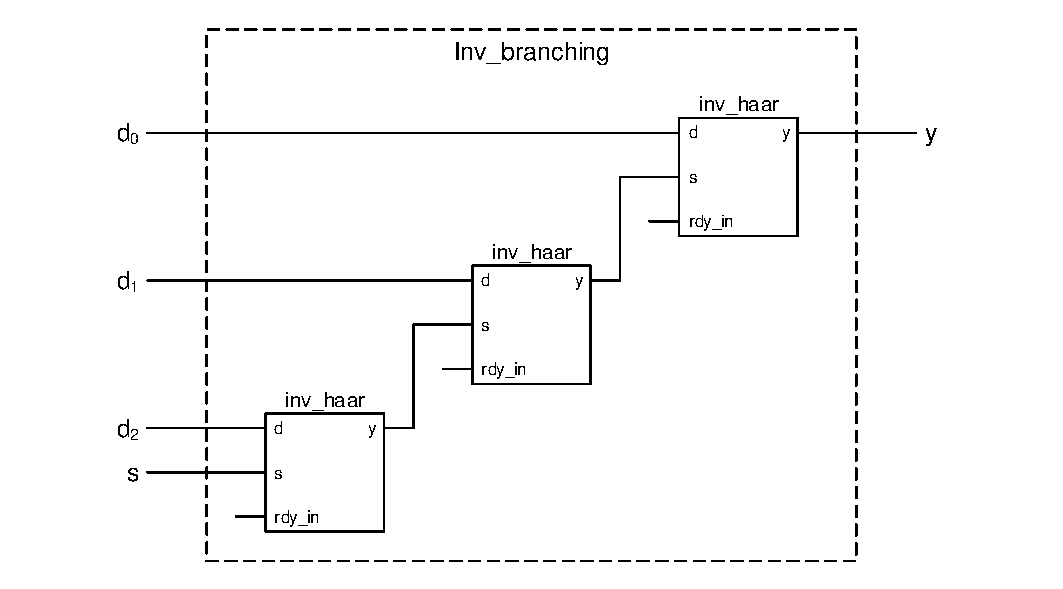
\includegraphics[scale=0.7]{inv_branching.pdf}
\end{figure}

\end{frame}

\begin{frame}
\frametitle{Pipeline}

	\centering
	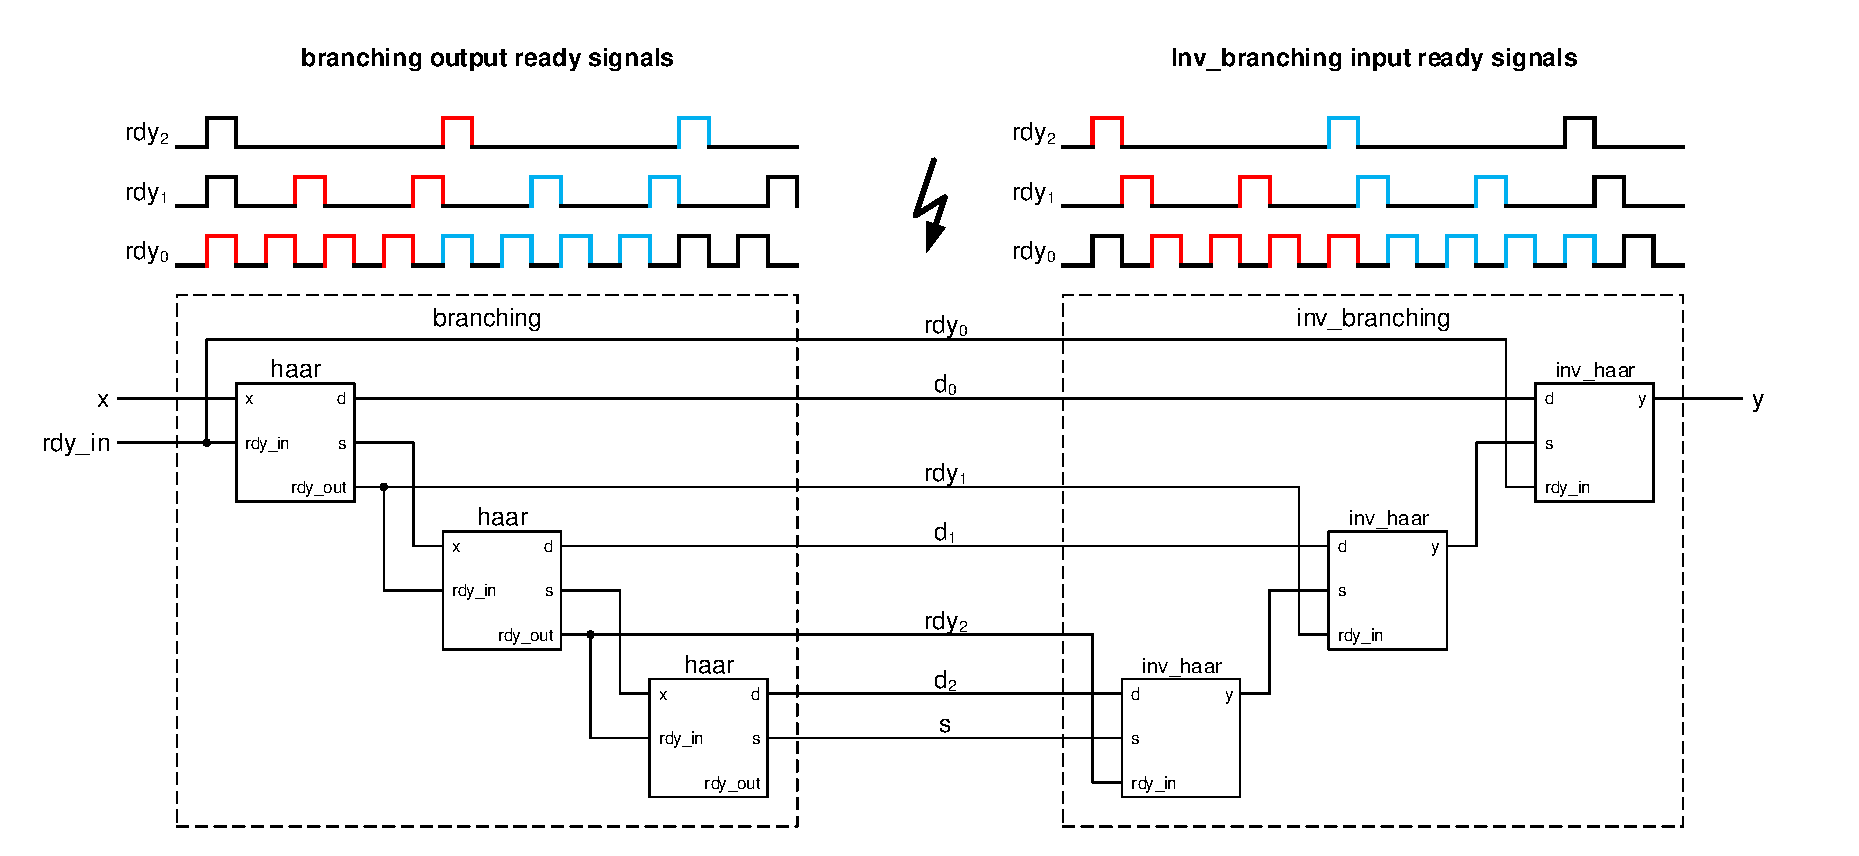
\includegraphics[scale=0.45]{main.pdf}

\end{frame}

\begin{frame}

\frametitle{Pipeline}

	\centering
	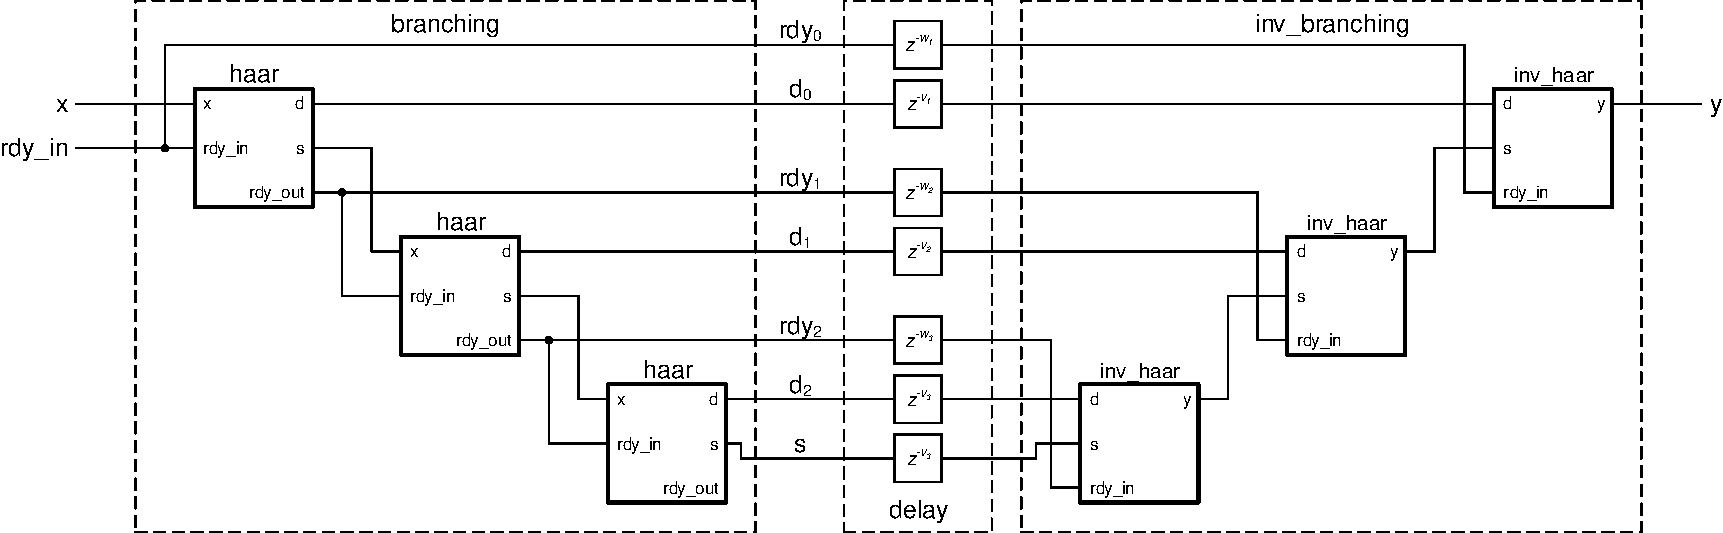
\includegraphics[scale=0.45]{main_delay.pdf}

\end{frame}





\section{VHDL Simulation and Testing}
\begin{frame}
\frametitle{Testing workflow}
	\centering
	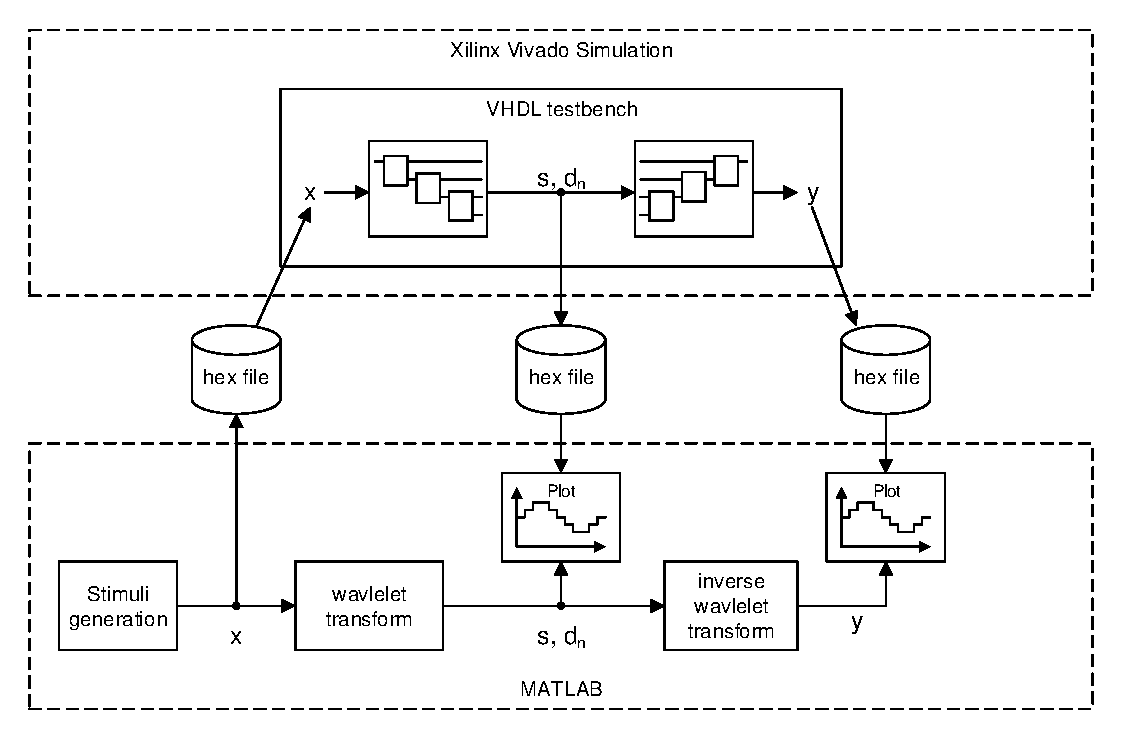
\includegraphics[scale=0.6]{vhdl_sim.pdf}
	
\end{frame}

\begin{frame}
\frametitle{Coefficients after branching}
	\centering
	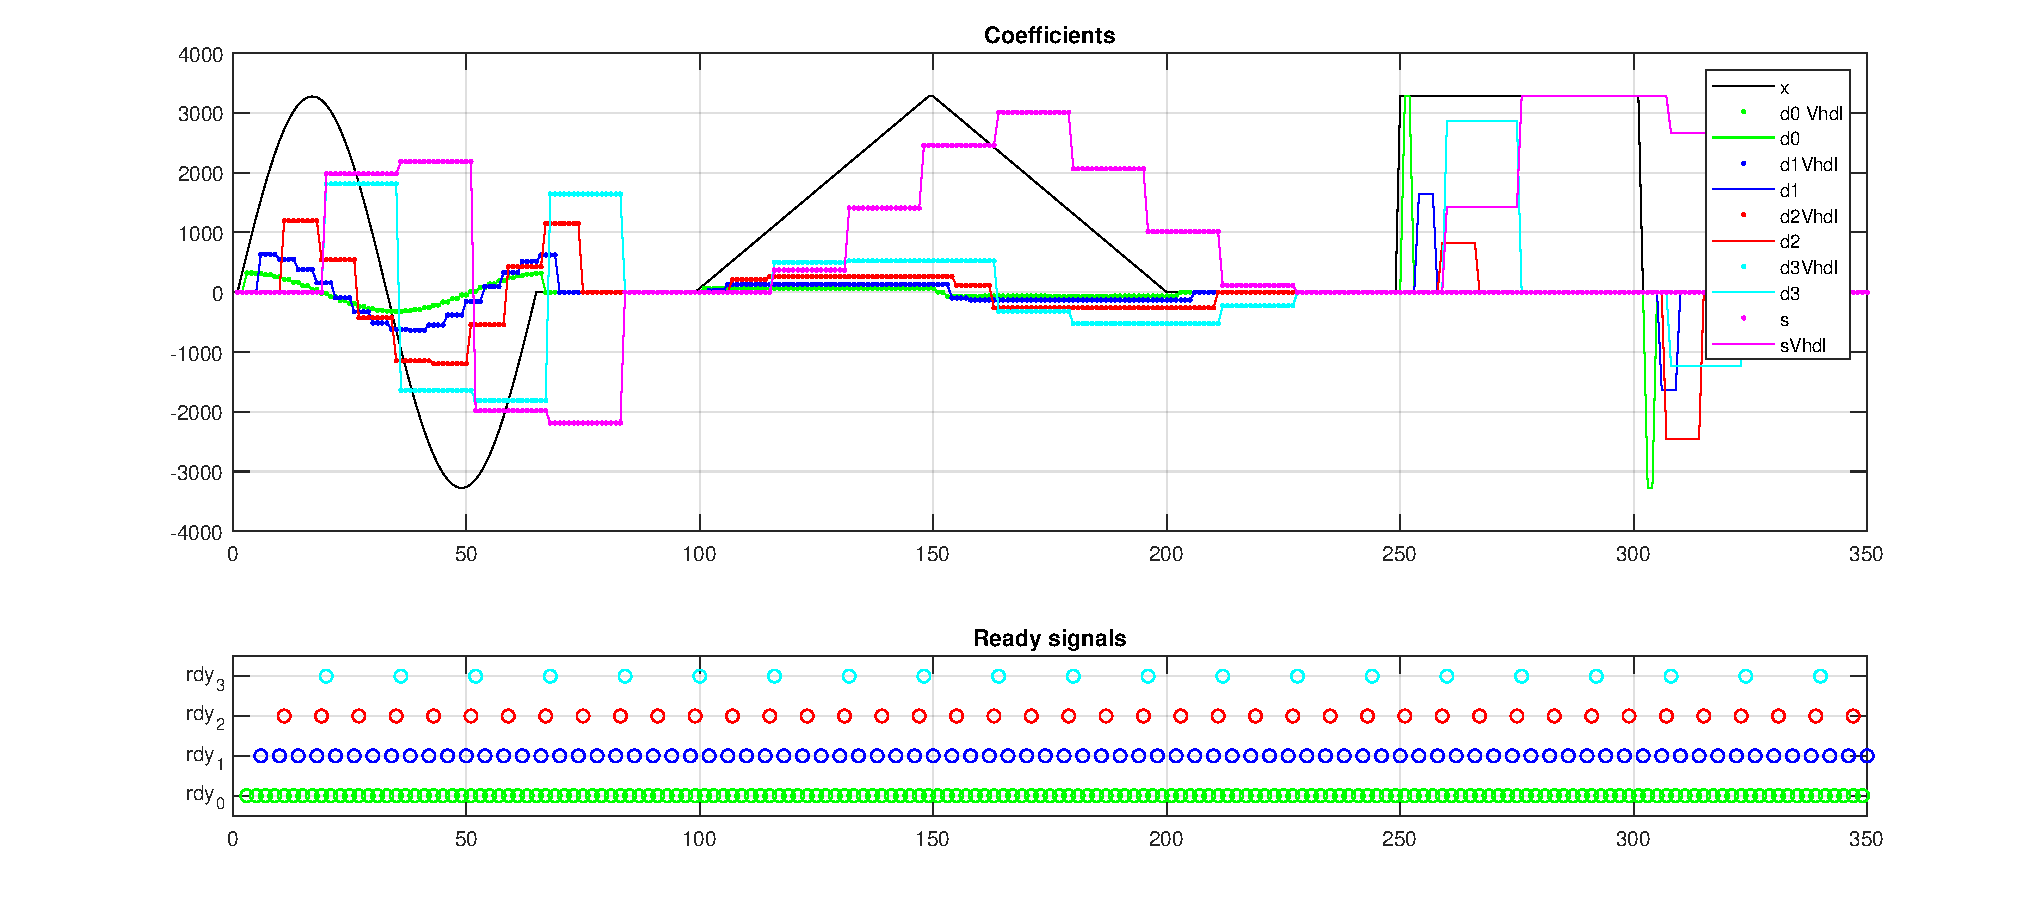
\includegraphics[scale=0.42]{coefs.pdf}
\end{frame}

\begin{frame}
\frametitle{Coefficients after delay}
	\centering
	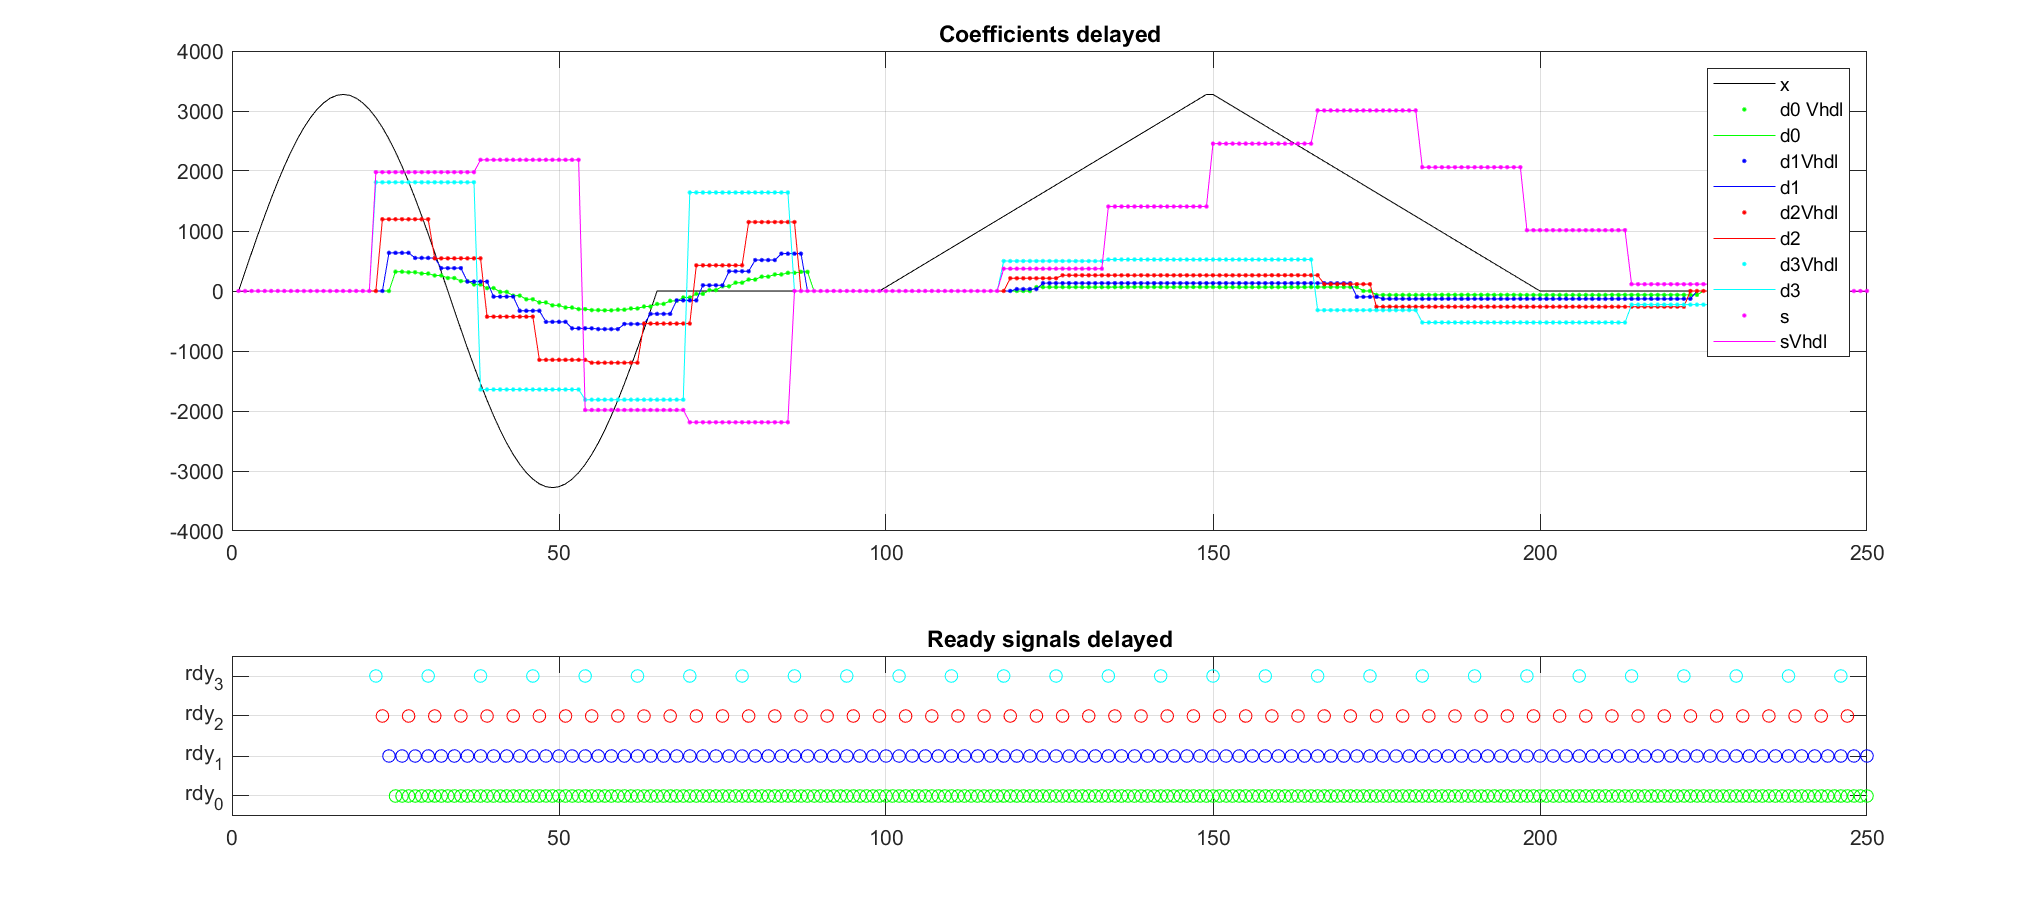
\includegraphics[scale=0.42]{coefs_delayed.pdf}
\end{frame}

\begin{frame}
\frametitle{Debranching visualization}
\centering
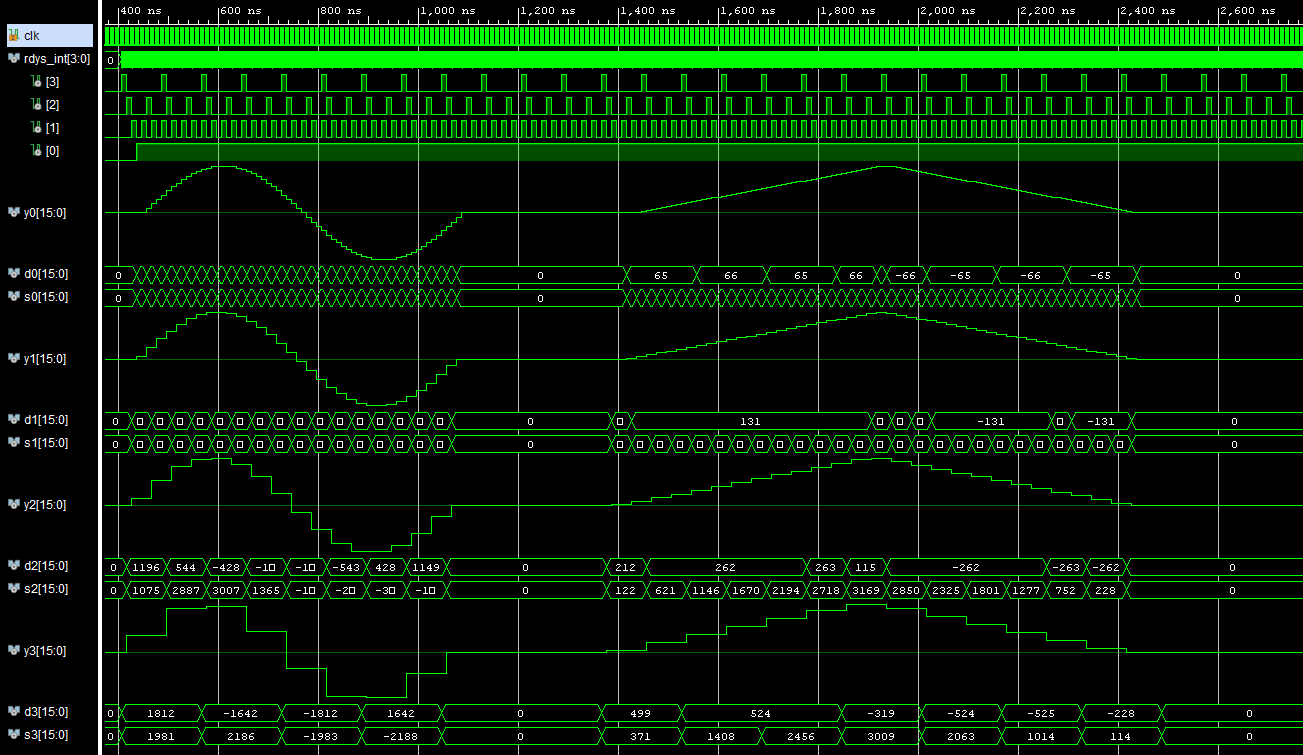
\includegraphics[width=\linewidth]{inv_branching_screenshot.PNG}
\end{frame}

\begin{frame}
\frametitle{Output}
	\centering
	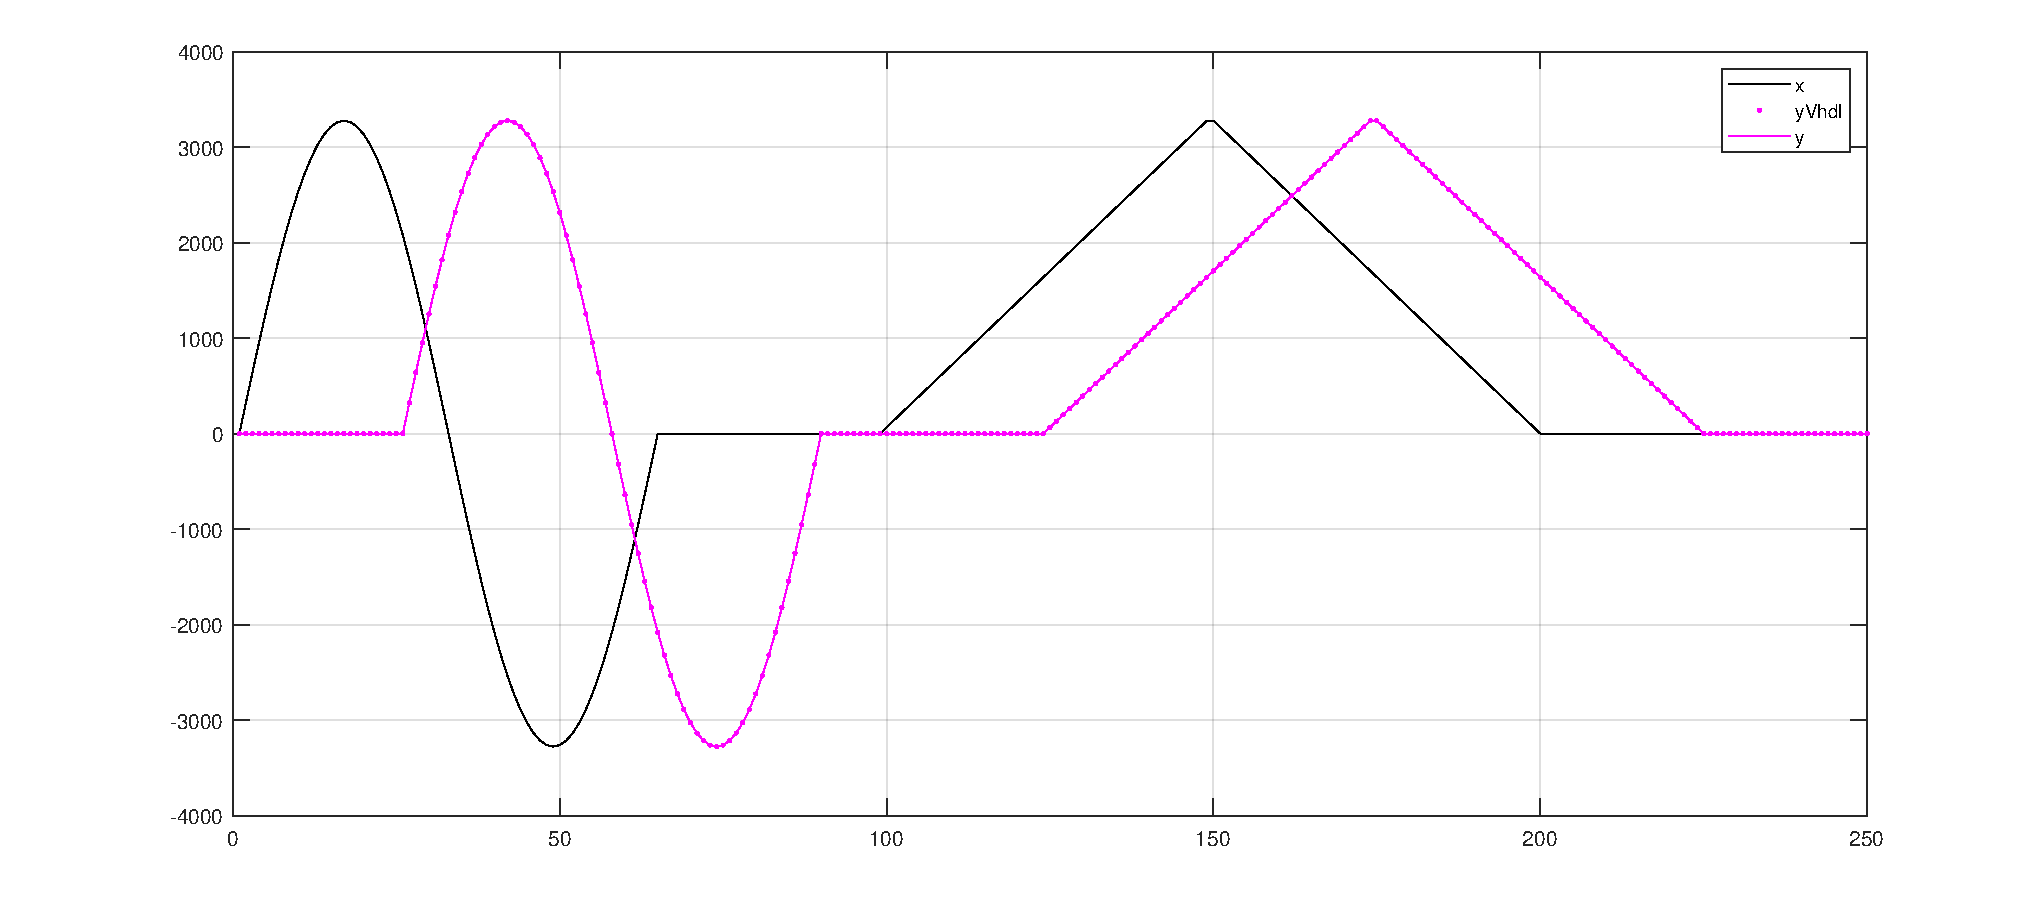
\includegraphics[scale=0.42]{output.pdf}
\end{frame}


\begin{frame}
\frametitle{DB4}
\centering
	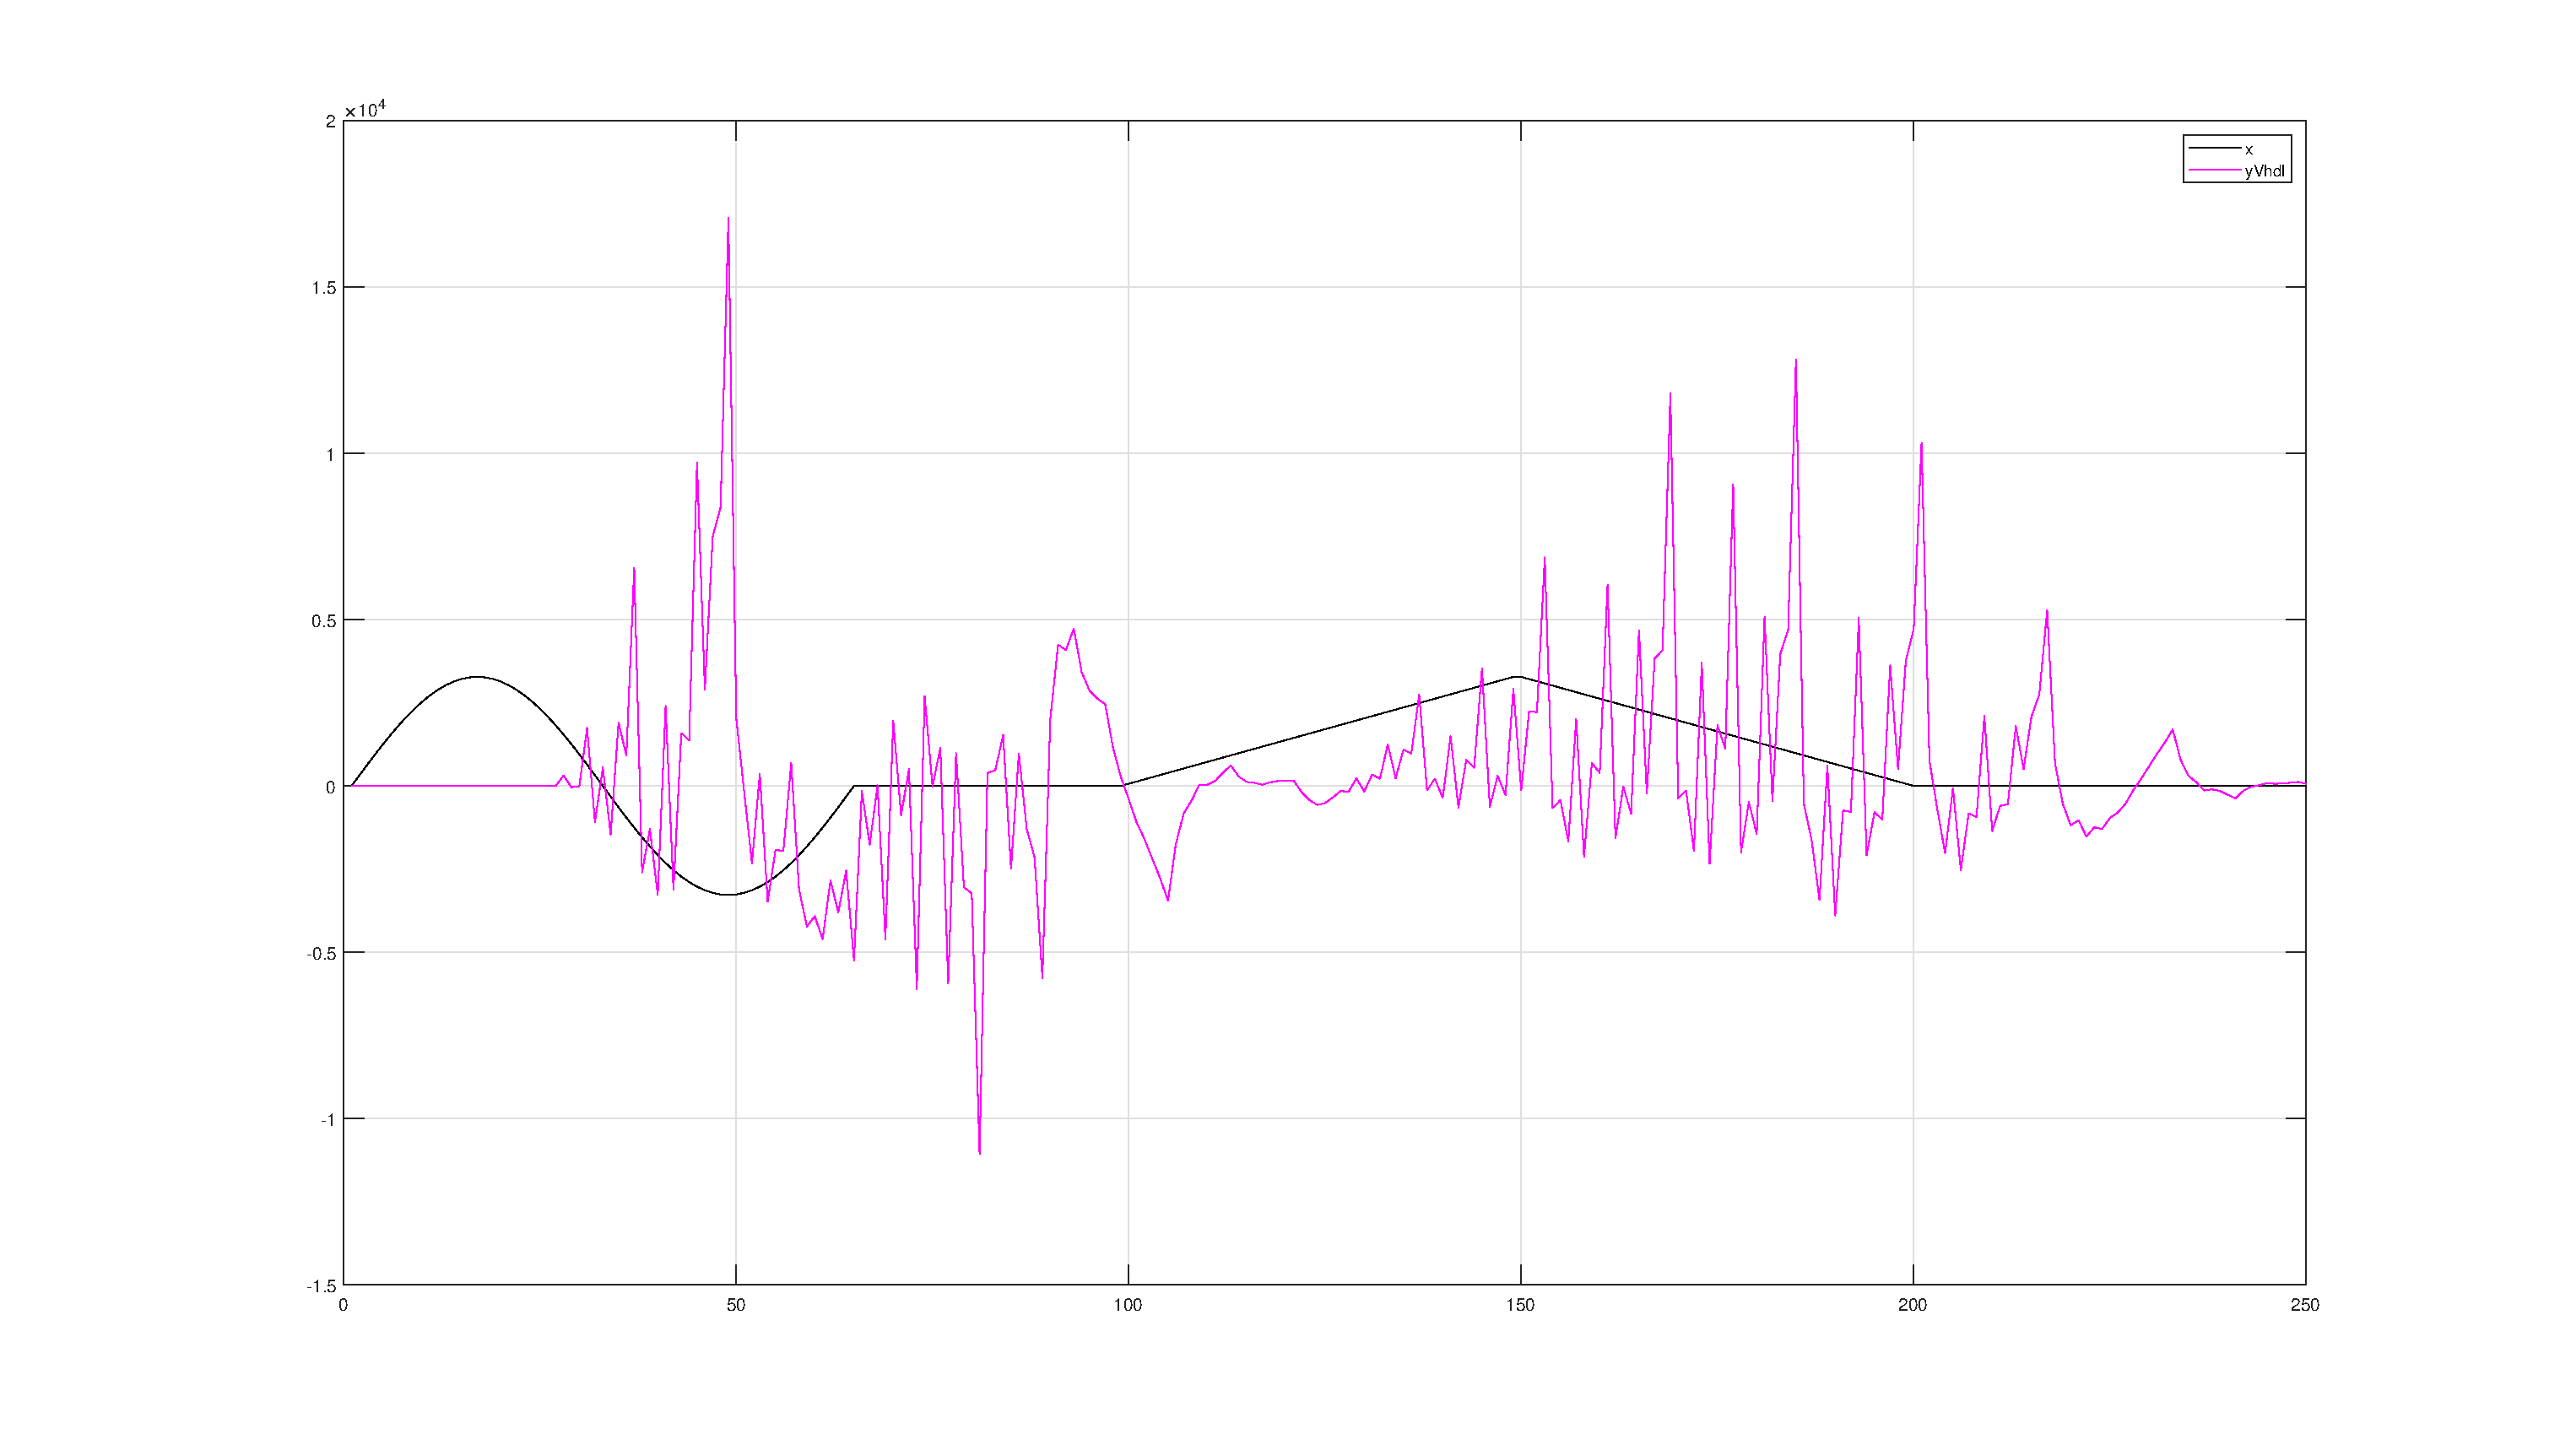
\includegraphics[scale=0.29]{db4.eps}
\end{frame}











%%%%%%%%%%%%%%%%%%%%%%%%%%%%%%%%%%%%%%%%%%%


\if 0

\section{Modell} 
\begin{frame}
	\frametitle{Modell}
	\begin{figure}
		\includegraphics[scale=1]{Model.eps}
	\end{figure}
\end{frame}

\subsection{Energiehaushalt}
\begin{frame}
\frametitle{Energiehaushalt}
\begin{itemize}
	\item[] Absorbierte Leistung
	\begin{equation}
	P_{in} = \sigma T_{\astrosun}^4 \left( \frac{R_{\astrosun}}{A_{planet}} \right) ^2 \cdot (1-\alpha)
	\end{equation}
	\pause
	
	\item[] Abgestrahlte Leistung
	\begin{equation}
	P_{out} = (4 \pi R^2 \sigma T^4)(1 - \beta)
	\end{equation}
	\pause
	
	\item[] Albedo
	\begin{equation}
	\alpha(C) = (0.55 \cdot C) + 0.10;
	\end{equation}
	\pause
	
	\item[] Treibhauseffekt
	\begin{equation}
	\beta(H) = 0.6 \cdot H
	\end{equation}
\end{itemize}
\end{frame}




\subsection{Wasserkreislauf}

\begin{frame}
	\frametitle{Wasserkreislauf}
	\begin{itemize}
		\item[] Wasserdampfbildung
			\begin{equation}
			\xi_4 (P_{in})
			\end{equation} 
		\pause
		\item[] Wolkenbildung
			\begin{equation}
			\xi_5 \left( H \frac{dT}{dh} \right)
			\end{equation}
		\pause
		\item[] Wolkenabbau 
		 	\begin{equation}
			\xi_6 (C)
			\end{equation}
	\end{itemize}
\end{frame}

\begin{frame}
	\frametitle{Wasserkreislauf}
	\begin{itemize}
	
		\item[] Wasserkreislauf
			\begin{equation}
				\begin{matrix}			
					\dot{H} = & \xi_4 P_{in}(C) & - \xi_5  H \frac{dT}{dz} & \\
					\dot{C} = &                 &   \xi_5  H \frac{dT}{dz} & - \xi_6 C
				\end{matrix}	
			\end{equation}
	
		\pause	
	
		\item[] Temperaturgradient
			\begin{equation}
				\frac{dT}{dz} \approx \Delta T
			\end{equation}
		
		\pause		
		
		\item[] Eingesetzt
			\begin{equation}
				\begin{matrix}			
					\dot{H} = & \xi_4 P_{in}(C) & - \xi_5 H \Delta T & \\
					\dot{C} = &                 &   \xi_5 H \Delta T & - \xi_6 C
				\end{matrix}	
			\end{equation}			
		
	\end{itemize}
\end{frame}

\subsection{Temperaturgradient}

\begin{frame}
	\frametitle{Temperaturgradient}
	\begin{itemize}
	
		\item[]Wasser kondensiert  $\rightarrow$ Niedriger Gradient
		
		\item[]Wärmere Luft $\rightarrow$ mehr Kondensation
	
	
		\item[]
		\begin{equation}
			\Delta T = \xi_3 \frac{1}{TC}
		\end{equation}
	
	
%		\item[] Oberflächentemperatur	
%			\begin{equation}
%			\dot{T_S} = p_1 \left( P_{in}(C) - P_{out}(T_S, H) \right)
%			\end{equation}
%		\item[] Tropopausentemperatur
%			\begin{equation}	
%			\dot{T_T} = p_2 \left( P_{in}(C) \cdot H \right) - P_{blackbody}(T_T) - p_3 \left( (T_T - T_S) \cdot H \right)
%			\end{equation}		
		
	\end{itemize}
\end{frame}

\subsection{Zusammengefasste Gleichungen}

\begin{frame}
\frametitle{Zusammengefasste Gleichungen}
\begin{itemize}
	\item[] Zusammengefasst
\begin{equation}
\left|
\begin{matrix}
\dot{T} = &  & \xi_1 \left(P_{in}(C) - P_{out}(T, H) \right) &\\
\dot{H} = & \xi_4 P_{in}(C) & - \xi_5 H \Delta T & \\
\dot{C} = &                 &   \xi_5 H \Delta T & - \xi_6 C
\end{matrix}
\right|
\end{equation}
	\pause
	\item[] Mit limitierenden Termen
\begin{equation}
\left|
\begin{matrix}
\dot{T} = & & \xi_1 \left(P_{in}(C) - P_{out}(T, H) \right) &\\
\dot{H} = & \xi_4 P_{in}(C) & - \xi_5 (H + H^9) \Delta T & \\
\dot{C} = &                 &   \xi_5 (H + H^9) \Delta T & - \xi_6 (C + C^5)
\end{matrix}
\right|
\end{equation}	
	
%\begin{equation}
%\left|
%\begin{array}{lcl}
%\dot{T}_S = p_1 \left( P_{in}(C) - P_{out}(T_S, H) \right) \\
%\dot{T}_T = p_2 \left( P_{in}(C) \cdot H \right) - P_{blackbody}(T_T) - p_3 \left( (T_T - T_S) \cdot H \right) \\
%\dot{C} = p_4 \left( (H + H^9)(T_S - T_T) \right) - p_5 (C + C^5) \\
%\dot{H} = p_5 \left(P_{in} \right) - p_4 \left( (H + H^9 )(T_S - T_T) \right)
%\end{array}
%\right|
%\end{equation}

\end{itemize}
\end{frame}

\section{Simulationsergebnisse}

\subsection{Temperatur}
\begin{frame}
	\frametitle{Temperatur}
		\begin{figure}
			\includegraphics[width=0.9\linewidth]{Matlab/figures/surfaceTemperature.eps}
		\end{figure}
\end{frame}

\subsection{Luftfeuchtigkeit}
\begin{frame}
	\frametitle{Luftfeuchtigkeit}
		\begin{figure}
			\includegraphics[width=0.9\linewidth]{Matlab/figures/humidity.eps}
		\end{figure}
\end{frame}

\subsection{Wolkenabdeckung}
\begin{frame}
	\frametitle{Wolkenabdeckung}
		\begin{figure}
			\includegraphics[width=0.9\linewidth]{Matlab/figures/cloudCover.eps}
		\end{figure}
\end{frame}

\subsection{Albedo}
\begin{frame}
	\frametitle{Albedo}
		\begin{figure}
			\includegraphics[width=0.9\linewidth]{Matlab/figures/albedo.eps}
		\end{figure}
\end{frame}

\section{Fazit}
\begin{frame}
\frametitle{Fazit}
\begin{itemize}

	\item[$\bullet$] Ergebnisse gleichen dem heutigen Status
	\item[$\bullet$] Extremes Klima von Mars \& Venus vermutlich prädestiniert
	
	\vspace{5mm}
	
	\item[$\bullet$] Ergebnisse nur mit Vorsicht zu geniessen	
	\begin{itemize}
		\item[-] Nur Wasser simuliert
		\item[-] Andere Treibhausgase vernachlässigt
		\item[-] Chemische und Physikalische Vorgänge bei extremen Temperaturen
	\end{itemize}

	
\end{itemize}
\end{frame}

\section{Nächste Schritte}
\begin{frame}
\frametitle{Nächste Schritte}
\begin{itemize}

	\item[$\bullet$] Modell ausbauen
	\begin{itemize}
		\item[-] Vereisung
		\item[-] Tag- \& Nachtseite
		\item[-] Rotationsgeschwindigkeit
		\item[-] Mehr atmosphärische Gase
	\end{itemize}
	
\end{itemize}
\end{frame}

\fi

\end{document}